\section{Supplement: the development study}
\label{sec:supplementdev}
\label{sec:dev}

This section reports what was tried before the final tests, on the
development windows only. It shows how the final models were chosen and which
ideas from the literature did not help on these data. Every row is a section
of the results record, with its run folders.

\subsection{Breakfast at the Frat}
\label{sec:dev-frat}

\paragraph{Benchmarks}
On the three windows before the data set's end, seasonal naive scores 0.832,
the average of the last 8 weeks 0.756, LightGBM with price only 0.554 and
LightGBM with every recorded lever 0.447. The levers are worth a fifth of the
error: display, feature and price reduction carry information price does not.

\begin{figure*}[t]
\centering
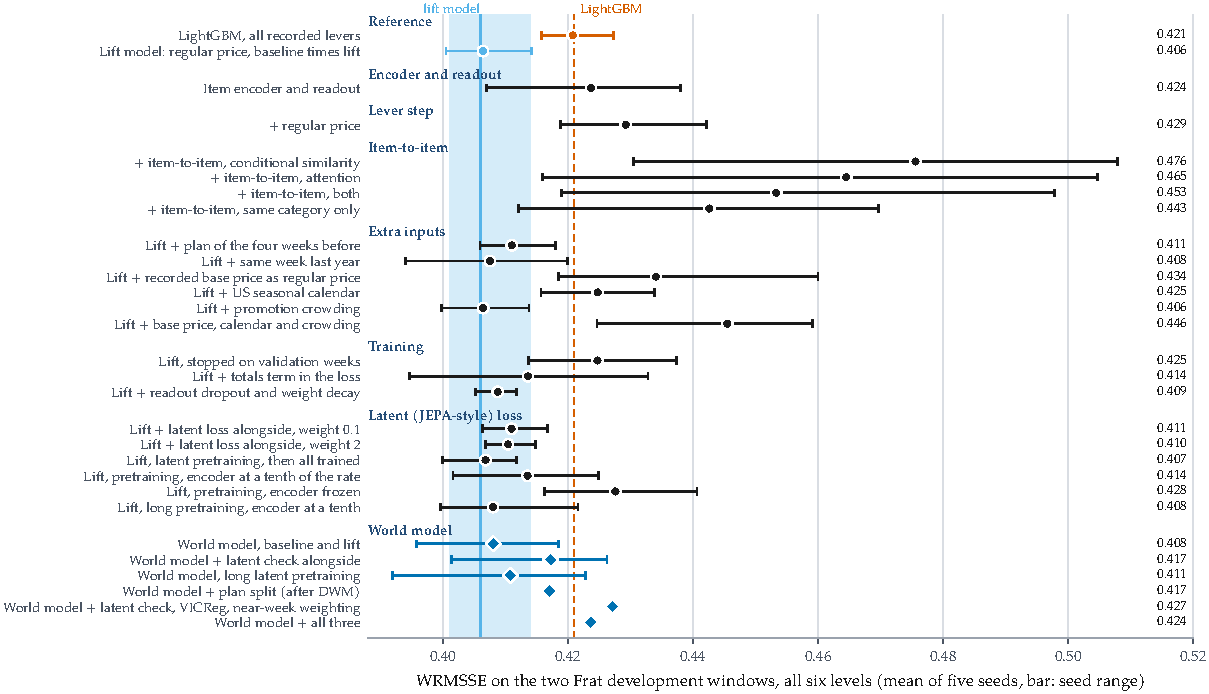
\includegraphics[width=\textwidth]{figs/fig_frat_dev.pdf}
\caption{\textbf{On Frat the gain came from building the forecast as a baseline
times a plan lift; item-to-item links, extra inputs, latent losses and the
roll-forward did not improve on it.} Each row is one configuration on the two
development windows, five seeds: mean (marker) and range (bar). Blue band: the
lift model's seed range; vertical lines: the lift model (0.406) and LightGBM
(0.421). Values below the lift model are in bold. Rows without a bar were
recorded as a mean only.}
\label{fig:fratdev}
\end{figure*}

\paragraph{What helped and what did not}
Figure~\ref{fig:fratdev} shows the configurations of the main comparisons on
Frat; Table~\ref{tab:record} lists the eleven other Frat configurations
screened, including the worst (0.458) and the best (0.400). Our item
encoder with a direct readout scored 0.424, level with LightGBM (0.421).
Building the forecast as a baseline under the nothing-planned plan times a lift
(the lift model) brought it to 0.406, better than LightGBM in all five runs and
with half the spread across seeds. Letting the 55 items in a store affect each
other, by conditional similarity, attention or both, made the forecast worse in
every version (0.443 to 0.476) and less steady; limiting it to items in the same
category narrowed the gap without closing it. Extra inputs did not help: the
plan of the four weeks before (0.411), the same week last year (0.408), the US
seasonal calendar (0.425), the count of items on promotion in the store (0.406)
and the recorded base price used as the regular price (0.434). The recorded
base price changes about twelve times a year per item and equals the shelf
price in every week without a promotion, so it is not a slow-moving regular
price.

\paragraph{Latent (JEPA-style) losses}
Following the JEPA literature~\cite{lecun2022,ijepa} and M-JEPA~\cite{mjepa}, we
added a loss that predicts the encoder's own state for the forecast weeks from
the state now and the plan, with a slowly updated copy of the encoder as the
target~\cite{byol}. No recipe beat the lift model: alongside the forecast loss
0.410 to 0.411, pretrained on the latent loss and then fine-tuned 0.407 to
0.414. With the encoder frozen after latent-only pretraining the model still
reached 0.428, so a state learned without any sales target carries most of the
forecast signal. Long pretraining followed by a slowed encoder gave the best
display-week error of any configuration (0.813 for the world model, against
0.817 for LightGBM).

\paragraph{The world model}
Rolling the state forward week by week under the plan scored 0.408, level with
the lift model on the overall score and on every lever. Three ideas from the
world-model literature, each at one untuned setting, did not help: keeping the
plan's effect apart from the no-plan state as in DWM~\cite{dwm} (0.417), a
latent check on each rolled step with a VICReg penalty~\cite{vicreg} and near
weeks weighted more as in TD-MPC2~\cite{tdmpc2} (0.427), and all three together
(0.424). Training changes did not help either: stopping at the best point on the
last 8 training weeks (0.425) took 8 of only 90 training weeks out of the
targets, and a term on summed totals in the loss (0.414) had no bias to fix,
since total forecasts were within 3\% of sales in every run. Readout dropout
with weight decay (0.409) was level and steadier, and was kept for the lift
model.

\input{generated/tab_tests}

\paragraph{Beyond accuracy}
Table~\ref{tab:tests} reports four further tests. \emph{New items}: with one
product in ten held out of training, the lift model borrowing the state and
level of the ten known items in the same store with the most labels in common
scored 0.890 on the new items, against 1.310 for LightGBM fitted on labels,
price and plan, and 1.510 for a forecast of zero; hiding the item label in a tenth of training
examples changed this little (0.879). On Dominick's analgesics,
where items carry no category or maker labels, borrowing failed (2.999 against
0.923): the method needs item attributes. \emph{Combination}: weighting the lift
model and LightGBM on a validation window gave the best Frat result of the study
(0.388), better than either part on display and circular weeks, because the two
make different errors in promoted weeks; on analgesics the combination was
level. Combinations were not carried to the final tests, which compare single
models. \emph{Plan A against plan B}: for pairs of weeks of the same item and
store with different plans, every model picked the week that sold more about
78\% of the time; LightGBM was marginally ahead. \emph{Unusual plans}: the
test as first defined, a lever mix under 2\% of all training rows, found no
such week in the windows, so it was redefined after that run as a mix the item
itself had run in under 2\% of its weeks. On those, no model degraded much and
LightGBM stayed ahead. The world model's ability to roll a plan forward did not
show as an advantage on these tests.

\subsection{Dominick's}
\label{sec:dev-dom}

\paragraph{Analgesics, the category used to set the models}
On analgesics, seasonal naive scored 1.274, the average of the last 8 weeks
0.723 and LightGBM 0.715. The lift model scored 0.676 on three seeds, and the
world model 0.667 once a totals term was removed from its loss: that term made
the total worse, pulling forecasts 8\% low (0.819 for the lift model). Training
four times longer without a stop broke the summed levels (1.473) while
item-by-store error barely moved, so a small bias in the same direction on
every item added up at the category total. The seasonal calendar with
promotion crowding made LightGBM worse (0.715 to 0.734) and, with a held price
as the regular price, took the lift model to 0.919 by the same route; the held
price alone was level (0.674). Item-to-item links did not help (0.697). Of the
world-model ideas that failed on Frat, the plan split improved item-by-store
error (0.707 to 0.693) and broke the total (0.687 to 0.793), and all three
together scored 0.730 against 0.667. Five seeds changed the picture: the
world model held (0.666) and LightGBM scored 0.702, but the lift model fell to
0.718, so a three-seed figure had flattered it.

\begin{figure*}[t]
\centering
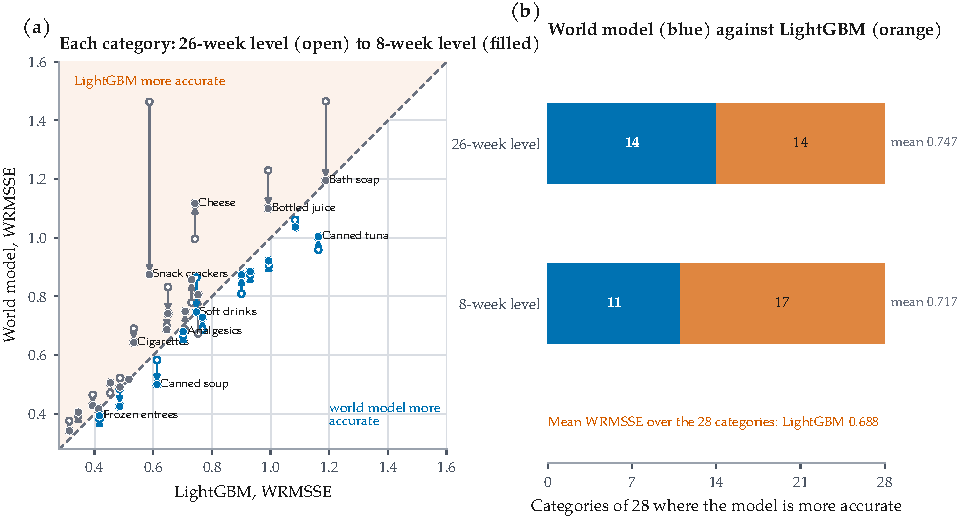
\includegraphics[width=\textwidth]{figs/fig_dom28.pdf}
\caption{\textbf{Run unchanged on all 28 Dominick's categories, the world model
set on analgesics failed badly in a few; taking each item's level from its last
8 weeks removed the worst failures but did not make it better than LightGBM on
average.} Development windows, one seed. \textbf{(a)} Each category's
WRMSSE for LightGBM (horizontal) and the world model (vertical), with the item
level from the last 26 weeks (open) and the last 8 weeks (filled); blue: the
world model is more accurate with the 8-week level. \textbf{(b)} Categories
where each model is more accurate, and the mean over the 28.}
\label{fig:dom28}
\end{figure*}

\paragraph{All 28 categories}
Run on all 28 categories with settings from analgesics, LightGBM was the most
accurate of the three in 14, the lift model in 5 and the world model in 9, with
mean WRMSSE 0.688, 0.784 and 0.747; on promoted weeks LightGBM was most accurate
in 24 of 27 (Figure~\ref{fig:dom28}, Table~\ref{tab:dom28}). Analgesics did not
generalise, which is why the paper reports every category. The failures (snack
crackers 1.463, bath soap 1.465, the lift model on soft drinks 1.406) sat at the
category total: item-by-store error was close to LightGBM's. On a six-store
sample of snack crackers (one seed, 800 training steps, recorded in
\texttt{docs/PAPER\_NOTES.md}) the cause was in-and-out and seasonal lines: items
recorded in 8 to 20 of the last 26 weeks were 8\% of sales and the lift model
forecast them at 9 times their sales, because the model set each item's level from its 26-week
average after the item had fallen away. Capping extreme weeks did little; taking
the level from the last 8 weeks removed most of it. On all 28 categories the
8-week level brought the world model's mean from 0.747 to 0.717 by removing the
large failures (snack crackers 1.463 to 0.874, bath soap 1.465 to 1.195), but it
was worse than the 26-week level in 15 of the 28 categories (cheese 0.996 to
1.116, cereals 0.673 to 0.805), the median rose from 0.689 to 0.736, and it beat
LightGBM in 10 categories against 14 before. It became the Dominick's default
because it removed the failures that decided the mean, not because it was
better in most categories. On eight categories the 8-week level beat a 4-week level in five for the world
model, and the 4-week level was better in five for the lift model, which shares
the setting; the lift model with an 8-week level broke bath soap (1.568 to
2.203), and with a 4-week level cigarettes (0.918 to 1.245). LightGBM, which sees short recent averages directly, does not have
the problem.

\input{generated/tab_dom28}

\paragraph{Peaks and dips}
In cheese, both our model and LightGBM under-forecast promoted weeks by about a
third in the holiday window, and cheese peaks do not sit on a fixed week
relative to the holidays: they follow the chain's promotion timing, which event
flags cannot place. Figure~\ref{fig:peaks} splits forecast against sales into
promoted weeks, the weeks just after a promotion, and ordinary weeks, for six
categories. The world model did not see the dip after a promotion where the dip
is large: it forecast 1.33 times sales after a promotion in snack crackers and
1.32 in soft drinks, against 0.92 and 0.90 for LightGBM. Feeding the model's own
sales forecast into the roll-forward, so that a promotion's sales could shape the
weeks after it, fixed the soft-drink dip (1.32 to 1.00) and made the overall
score worse in four of six categories. Weighting the loss by dollar sales and by
how far a week sits from the item's usual level fixed cheese promoted weeks
(1.21 to 1.00) and was worse overall in three categories. Both together were
worse overall than the world model in four categories (snack crackers 0.874 to
1.294, bottled juice 1.100 to 1.222, analgesics 0.679 to 0.901) and the best of
all models only in frozen entrees (0.377). Adding the normalised roll-forward to
the sales feedback put the snack-cracker forecast after a promotion right (0.97
of sales) and broke its category total (1.60; overall 1.268). In frozen entrees every
model, LightGBM included, forecast about 0.7 of sales after a promotion: there the
week after is stronger than any model expected.

\begin{figure*}[t]
\centering
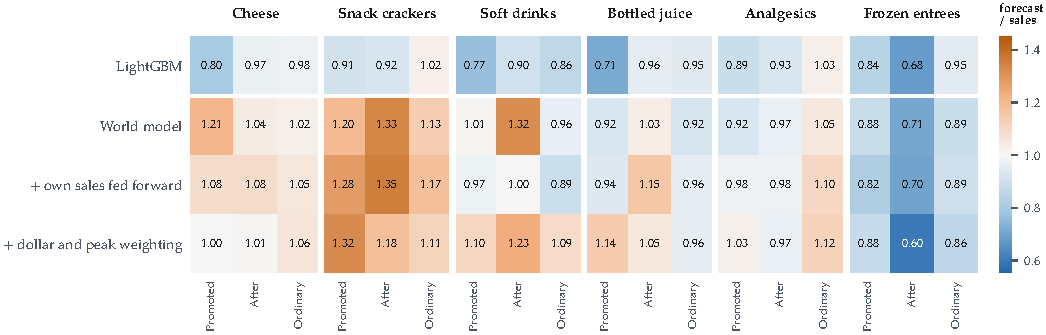
\includegraphics[width=\textwidth]{figs/fig_peaks.pdf}
\caption{\textbf{The world model over-forecast the weeks after a promotion where
shoppers had stocked up; the two fixes each repaired one category and hurt
others.} Forecast against sales (1.0 is right; orange over, blue under) in
promoted weeks, the weeks just after a promotion and ordinary weeks, Dominick's
development windows, one seed. Rows: LightGBM, the world model with the 8-week
level, with its own sales forecast fed forward, and with the loss weighted by
dollar sales and by peaks.}
\label{fig:peaks}
\end{figure*}

\paragraph{From the first world model to the one tested}
Figure~\ref{fig:ladder} follows the world model on the six categories through
the changes kept, three seeds each. Across seeds the first version was unsteady:
its range within a category was 0.04 to 0.38, against under 0.03 for LightGBM,
and on the mean LightGBM was ahead in five of six. Brand switching fixed what it
was built for: in snack crackers and soft drinks, where promoted weeks broke the
total, it was better on every seed (0.813 to 0.752, 0.902 to 0.789) and
item-by-store error improved too. Elsewhere it did not help: it was better on
no seed in cheese and frozen entrees and on one of three in bottled juice and
analgesics, and the mean was worse in cheese (1.088 to 1.111) and frozen
entrees (0.406 to 0.416). It was kept for all six. The fitted share of the summed lift that the category total keeps
(Figure~\ref{fig:ladder}g) is 0.00 to 0.66 in snack crackers, against about 0.9
in bottled juice, analgesics and frozen entrees: in snack crackers the summed
item lifts overstated the category total, and the fit took most of it back.
Where it comes out at 1.0 the step changes nothing, a built-in check. The
direction agrees with van Heerde, Gupta and Wittink's household
estimates~\cite{vanheerde2003}, but the share is fitted to make totals right; it
is not an estimate of switching. Normalising the rolled state, tried first on
one seed, was better in two categories, worse in three (analgesics 0.679 to
0.790, soft drinks 0.747 to 0.882) and level in one, and the record ruled it
out as a general fix. With switching and three seeds it narrowed the seed
range in five of six categories, but the mean was worse than switching alone in
snack crackers (0.752 to 0.830) and soft drinks (0.789 to 0.827). Added to
switching with three fits averaged (seed 1), it was better in four categories
and worse in cheese (0.921 to 0.983) and snack crackers (0.722 to 1.806); three
fits averaged without it had broken bottled juice (1.170). It was kept because
the combination was the steadiest version. Averaging three fits per run with normalisation gave the
steadiest version (range 0.05 or less in five categories) and the candidate for
the final test: better than LightGBM on the three-seed mean in analgesics (0.621
against 0.701), frozen entrees (0.391 against 0.419) and soft drinks (0.743
against 0.759). One snack-cracker run of the three failed (1.806): its second
window's category total broke with promoted weeks forecast at 2.6 times sales
while item-by-store error stayed normal, so the summed promotion lift can still
run away on one fit in three. Twice the training steps, screened after the final
tests were fixed, was better in two categories, worse in two, level in one and
mixed in one, and was not kept.

\begin{figure*}[t]
\centering
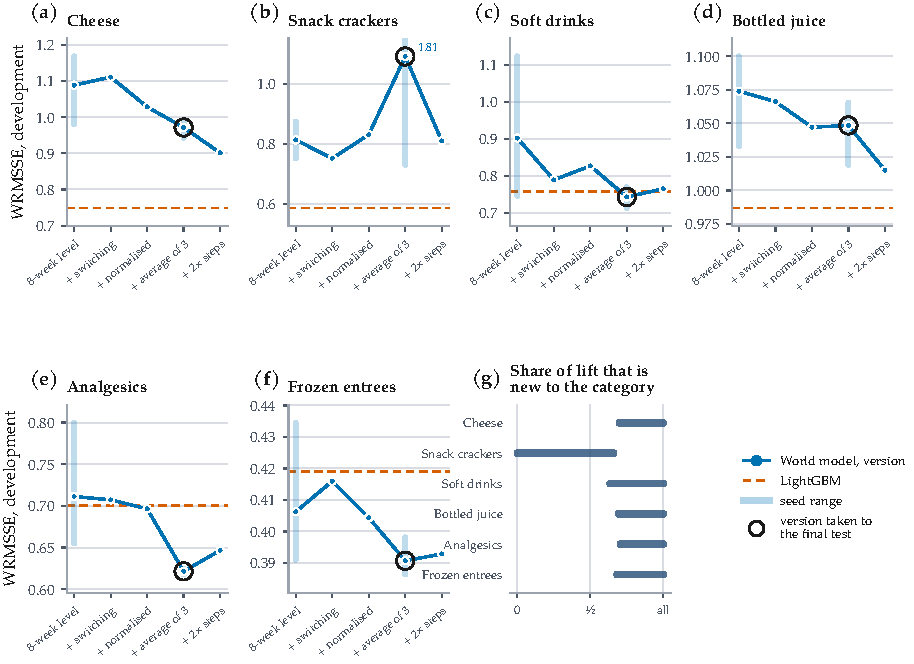
\includegraphics[width=\textwidth]{figs/fig_ladder.pdf}
\caption{\textbf{Brand switching, a normalised roll-forward and averaging three
fits took the world model past LightGBM in three of six categories on the
development windows, and the switching step learned how much of a promotion's
lift is new to the category.} \textbf{(a--f)} Development WRMSSE of each version,
three-seed means; shaded bars: seed range of the first version and of the one
taken to the final test (circled); dashed: LightGBM. \textbf{(g)} The fitted share of the summed promotion lift that the category
total keeps, the split that makes category totals fit best (not an estimate of
switching), range over runs.}
\label{fig:ladder}
\end{figure*}

\paragraph{Other changes}
Showing the model both its 26-week and its recent levels as inputs, instead of
setting its scale by the recent level, was the best world-model version in four
of ten categories but did not fix snack crackers (1.515) or soft drinks (1.069):
the model did not learn to switch to the recent level when the long level still
set its scale. Item role labels (new line, in-and-out, volume driver, long tail,
high-low, promotion-responsive, core), assigned from each item's own sales before
the windows, moved LightGBM by at most 0.013, since it reads the same information
from its history, and moved the world model in both directions; letting the role
pick the level broke snack crackers (2.422). We did not call the volume drivers
key value items, since a key-value-item list rests on shopper price perception,
which these data do not record.

\subsection{M5}
\label{sec:dev-m5}

\input{generated/tab_m5dev}

On the M5 practice window (Table~\ref{tab:m5dev}), the item encoder with a
direct readout scored 0.699 over five seeds against 0.715 for LightGBM, and the
lift and world models were level with LightGBM over three seeds (0.713 and
0.707). Normalising the rolled state was the one change that separated the world
model: 0.656, with its worst seed (0.675) better than the best seed without it
(0.679), all of the gain at the totals and the seed range cut from 0.071 to
0.029. On Dominick's 8 weekly steps it was worse in three of six categories
at one seed (\S\ref{sec:dev-dom}), which fits the reading that it stops the
state drifting over a long roll and has little to stop over a short one.
Averaging three fits did not help on M5 (0.665), where single fits were already
steady.

After the official test month, an error analysis of the world model found its
2.6\% excess in Foods (+3.9\%), in one store (CA\_3, +7.5\%), and on Sundays and
Mondays (+5.1\%, +6.4\%), not growing with the horizon. Grouped by sales in the
28 days before the test, the excess came from items that had been selling fast
(+5.4\% and +6.1\% on items selling 3 to 10 and over 10 a day). Four changes
were screened on the practice window under rules written before screening:
weekday as seven inputs, event kinds, twice the training steps, and the item's
level against its past-year level. None beat the original
(Table~\ref{tab:m5dev}), so there was no second version. On the practice window
every version under-forecast by 4\% to 6\%, while on the test month the world
model over-forecast by 2.6\%: the sign of the level error changed between
adjacent months, so a fix tuned on one would not carry to the next. That
finding is what led to the confirmation months of \S\ref{sec:res-final}.

\subsection{Every change and run in the record}
\label{sec:dev-record}

Every run is recorded in \texttt{results/README.md}, with its configuration and
run folders. Table~\ref{tab:changes} scores every change to a model setting
that has saved runs against the configuration it changed: \rcount{changen}
changes over \rcount{changepairs} comparisons. Several changes that were kept
won about half their comparisons or fewer; the text above gives the reason each
was kept. Table~\ref{tab:record} lists the results in the record not shown in
the figures and tables above, and the configurations that were written and
never run on full data.

\begin{table*}[t]
\centering
\caption{\textbf{Every change to a model setting with saved runs, scored against the configuration it changed;
most were lower in error in at most half their comparisons, including some that were kept.} A comparison is two
configurations with the same data, windows and every other setting, scored on the windows and seeds both ran
(overall WRMSSE, development windows, from the audit of the saved runs). Comparisons: the number of such pairs
(categories, data sets or base configurations); lower: how many the change won. With it and without: mean WRMSSE
over the pairs. Kept: whether the change is in the models of the main text. Loss changes are in
Table~\ref{tab:losses}; averaging fits, the stock term and runs without saved models are in the text and
Table~\ref{tab:record}. Built by \texttt{scripts/change\_ledger.py}.}
\label{tab:changes}
\footnotesize
\begin{tabular}{p{0.36\textwidth}p{0.15\textwidth}rrrrl}
\toprule
\textbf{Change} & \textbf{Tested on} & \textbf{Comparisons} & \textbf{Lower} & \textbf{With it} &
\textbf{Without} & \textbf{Kept} \\
\midrule
Item level from the last 8 periods, against the whole history window & Dominick's & 36 & 17 & 0.799 & 0.804 & Yes (Dominick's) \\
Normalised roll-forward & Dominick's, M5 & 19 & 10 & 0.845 & 0.832 & Yes (M5, Dominick's) \\
Own forecast fed into the roll-forward & Dominick's & 18 & 4 & 0.910 & 0.816 & No \\
Item level from the last 4 periods, against the whole history window & Dominick's & 16 & 12 & 0.938 & 0.987 & No \\
Item level from the last 8 periods, against the last 4 & Dominick's & 16 & 8 & 0.966 & 0.938 & No \\
Brand switching & Dominick's & 12 & 7 & 0.797 & 0.832 & Yes (Dominick's) \\
Both levels as inputs, scaled by the 26-week level (against the 8-week level) & Dominick's & 6 & 2 & 0.946 & 0.818 & No \\
Level window set by the item's role & Dominick's & 6 & 1 & 1.125 & 0.884 & No \\
Roll-forward through the plan (world model against lift model) & Dominick's, Frat, M5 & 6 & 2 & 0.504 & 0.504 & Yes (world model) \\
Plan split into regular and promoted parts & Dominick's, Frat & 5 & 1 & 0.538 & 0.520 & No \\
More training steps & Dominick's, Frat, M5 & 3 & 1 & 0.844 & 0.578 & No \\
Plan of earlier periods as inputs & Frat & 2 & 0 & 0.414 & 0.407 & No \\
Year-ago sales as an input & Frat & 2 & 0 & 0.413 & 0.409 & No \\
Event kinds as inputs & M5 & 1 & 1 & 0.646 & 0.653 & No \\
Longer history and training period & Frat & 1 & 0 & 0.413 & 0.406 & No \\
New-item start from similar items & Frat & 1 & 1 & 0.461 & 0.594 & New-item test only \\
Past-year level & M5 & 1 & 0 & 0.680 & 0.646 & No \\
Readout dropout and weight decay & Frat & 1 & 0 & 0.409 & 0.406 & Yes (Frat lift model) \\
Recorded base price as the regular price & Frat & 1 & 0 & 0.434 & 0.406 & No \\
Regular price held for more periods & Dominick's & 1 & 1 & 0.674 & 0.676 & No \\
Unknown-item labels in training & Frat & 1 & 1 & 0.459 & 0.461 & No \\
Weekday and event kinds as inputs & M5 & 1 & 1 & 0.646 & 0.646 & No \\
Weekday as seven inputs & M5 & 1 & 0 & 0.653 & 0.646 & No \\
\bottomrule
\end{tabular}
\end{table*}


\begin{table*}[t]
\centering
\caption{\textbf{Results in the record not shown elsewhere in the paper, and
configurations never run on full data.} Overall WRMSSE on the development
windows, lower is better; ``against'' gives the configuration it changed. Frat:
five seeds; analgesics: three seeds; other Dominick's rows: one seed. Values
transcribed from \texttt{results/README.md}.}
\label{tab:record}
\footnotesize
\renewcommand{\arraystretch}{1.1}
\begin{tabular}{p{0.50\textwidth}p{0.12\textwidth}>{\raggedright\arraybackslash}p{0.30\textwidth}}
\toprule
\textbf{Run} & \textbf{Where} & \textbf{Result} \\
\midrule
Item encoder and readout, whole stores drawn in training & Frat & 0.430 against 0.424 \\
Item encoder and readout, 10,000 steps & Frat & 0.432 against 0.424 \\
Lever step with the latent loss alone & Frat & 0.428 against 0.429 \\
Lift model, 52 weeks of history & Frat & 0.413 against 0.406 \\
Lift model, plan of the four weeks before and the same week last year & Frat & 0.418 against 0.406 \\
LightGBM with the seasonal calendar and promotion crowding & Frat & 0.426 against 0.421 \\
Lift model with validation stop, totals term, dropout and weight decay together & Frat & 0.445 against 0.406 \\
Lift model, latent pretraining, encoder at a tenth of the rate, latent loss kept on & Frat & 0.415 against 0.406 \\
World model, long latent pretraining, with validation stop and totals term & Frat & 0.458 against 0.408 \\
LightGBM, average of five fits & Frat & 0.417 against 0.421 \\
Lift model, average of five fits & Frat & 0.400 against 0.406; the best Frat result of any single model family, not carried to the final tests (the record gives no reason) \\
\midrule
Lift model, all training fixes with long training & Analgesics & 0.716 against 0.676 \\
World model with the totals term, and with the best Frat recipe & Analgesics & 0.732 and 0.729 against 0.667 \\
World model, latent check, VICReg penalty and near-week weighting & Analgesics & 0.685 against 0.667 \\
\midrule
World model with switching, three fits averaged, without the normalised roll-forward & 6 categories & Bottled juice 1.170 against 1.066 \\
\midrule
World model, full-length training, with seasonal inputs, and with a dollar-weighted loss & 4 categories & Configured (job \texttt{dominicks\_seasonal\_long}); not run on full data \\
World model, unit-volume weighted loss & 8 categories & Configured (job \texttt{dominicks\_units\_loss}); not run on full data. On a six-store sample (lift model, 800 steps) it cut the snack-cracker over-forecast from 1.63 to 1.39 \\
\bottomrule
\end{tabular}
\end{table*}

% =====================================================================
